\documentclass[
a4paper, % Paper size, use either a4paper or letterpaper
12pt, % Default font size, the template is designed to look good at 12pt so it's best not to change this
%unnumberedsections, % Uncomment for no section numbering
]{article}
\usepackage[a4paper,top=1.2cm, bottom=1.6cm, left=1.6cm, right=1.6cm]{geometry}

\usepackage{cmap} % make PDF files searchable and copy-able
\usepackage[utf8]{inputenc}
\usepackage[english,russian]{babel}

\usepackage{amssymb,amsmath}
\renewcommand {\phi}{\varphi}
\usepackage{mathtext}

\usepackage{libertine}
\usepackage[libertine]{newtxmath}

\usepackage{graphicx} % Required for inserting images
\graphicspath{{./img/}} % Destination of images
\usepackage{subcaption}

\usepackage{hyperref}

\usepackage{xcolor}

% opening
\title{
	\textcolor{cyan}{Отчет о выполнении лабораторной работы 4.1.1}
	\\
	Изучение центрированных оптических систем
}
\author{Шубин Владислав, Байбулатов Амир}
%\date{Сентябрь 2023}

\begin{document}    
	
	\maketitle
	
	\section{Аннотация}
	В данной работе исследуются центрированные оптические системы. Центрирование производится во той причине, что, проходя через плохо отцентрированную систему, лучи света могут отклониться и пройти мимо экрана или глаза наблюдателя. Центрировать линзы следует как по высоте, так и в поперечном направлении (для чего линзы установлены на поперечных салазках). Для того, чтобы сознательно моделировать оптические инструменты, нужно знать фокусные расстояния линз, которые могут быть использованы в качестве объектива или окуляра модели. Фокусные расстояния тонких положительных линз проще всего найти с помощью вспомогательной зрительной трубы, установленной на бесконечность. При определении фокусного расстояния отрицательной линзы предметом служит изображение шкалы, которое даёт вспомогательная положительная линза.
	
	\newpage
	
	\section{Теоретические сведения}
	
	\subsection*{Определения фокусных расстояний}
	Формула тонкой линзы имеет вид
	\begin{equation}
		\frac{1}{F} = \frac{1}{f} + \frac{1}{d}\, \text{ , где}
	\end{equation}
	\begin{itemize}
		\item $F$ -- фокусное расстояние,
		\item $f$ -- расстояния от предмета до линзы,
		\item $d$ -- расстояние от изображения до линзы.
	\end{itemize}
	
	Измерить фокусное расстояние тонкой собирающей линзы можно по Методу Бесселя: рис. \ref{Bessel scheme} и формула \eqref{Bessel eq}.
	\begin{equation}
		F = \frac{L^2 - l^2}{4L}
		\label{Bessel eq}
	\end{equation}
	
	\begin{figure}[h!]
		\centering
		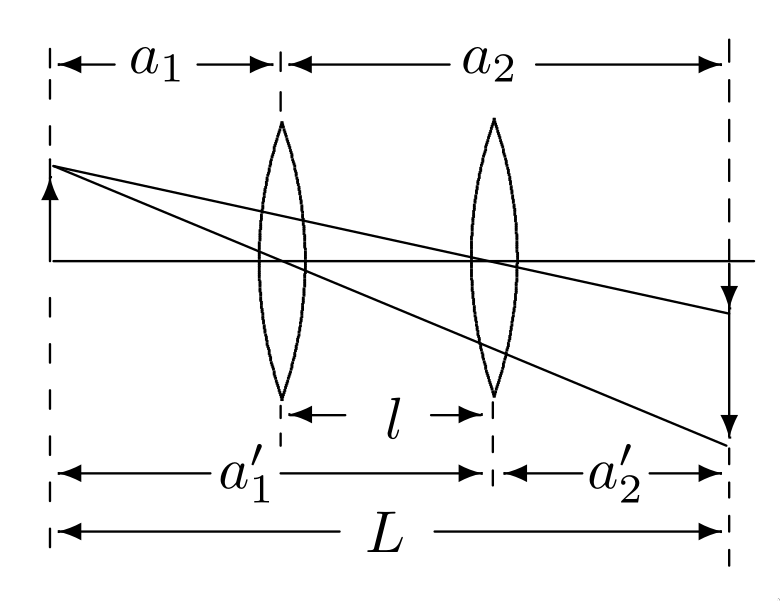
\includegraphics[scale=0.3]{measurement_collecting_lens.png}
		\caption{Схема измерения фокуса тонкой собирающей линзы по методу Бесселя}
		\label{Bessel scheme}
	\end{figure}
		

	Также фокусное расстояние тонкой собирающей линзы можно измерить с помощью зрительной трубы, настроенной на бесконечность. Если расположить линзу между предметом и трубой и найти четкое изображение предмета, то расстояние от линзы до предмета будет равно фокусному рис. \ref{Tube_collective}.
	
	\begin{figure}[h!]
		\centering
		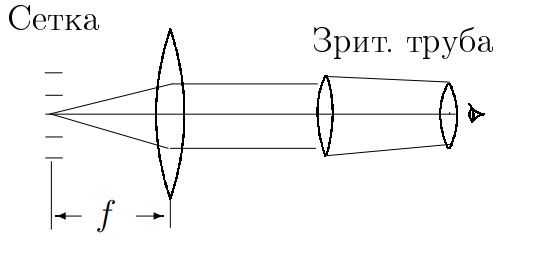
\includegraphics[scale=0.8]{tube_collective.jpg}
		\caption{Определение фокусного расстояния собирающей линзы}
		\label{Tube_collective}
	\end{figure}
	
	\newpage

	Для определения расстояния тонкой рассеивающей линзы воспользуемся схемой на рис. \ref{focus_scattering} и формулой тонкой линзы. Также можно воспользоваться зрительной трубой, настроенной на бесконечность. Если расположить предмет у нее в фокусе, то изображение переместиться в бесконечность, что можно проверить с помощью зрительной трубы рис. \ref{Tube_scattering}.
	
	\begin{figure}[h!]
		\centering
		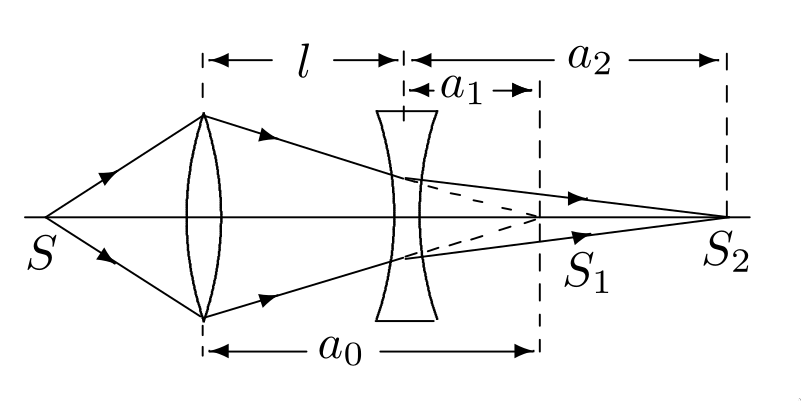
\includegraphics[scale=0.4]{measurement_scattering_lens.png}
		\caption{Определение фокусного расстояния рассеивающей линзы}
		\label{focus_scattering}
	\end{figure}
	
	\begin{figure}[h!]
		\centering
		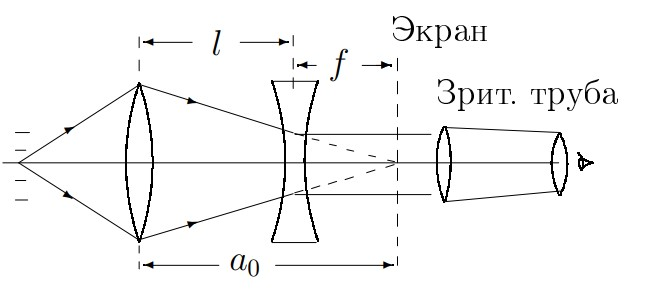
\includegraphics[scale=0.8]{tube_scattering.jpg}
		\caption{Определение фокусного расстояния рассеивающей линзы}
		\label{Tube_scattering}
	\end{figure}
	
	Существует также метод Аббе: схема рис. \ref{Abbe} и формула \eqref{Abbe eq}.
	
		\begin{figure}[h!]
		\centering
		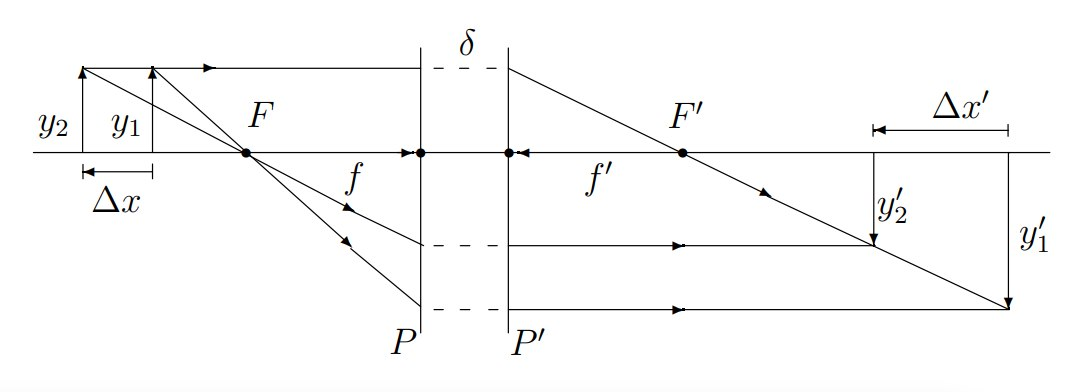
\includegraphics[scale=0.6]{Abbe.jpg}
		\caption{Измерение фокусного расстояния по методу Аббе}
		\label{Abbe}
	\end{figure}
	
	\begin{equation}
		F = \frac{\Delta x}{y_1 / y_1' - y_2 / y_2'
		}
		\label{Abbe eq}
	\end{equation}
	
	\subsection*{Определение положения главных и фокальных плоскостей сложной оптической системы}
	
	Для нахождения главных плоскостей системы недостаточно знать фокусное расстояние, нужно определить ещё положения главных фокусов. Это можно сделать при помощи зрительной трубы, настроенной на бесконечность. Отложив от главных фокусов отрезки, равные фокусному расстоянию, можно найти положения главных плоскостей системы. При этом необходимо учитывать возможность различного взаимного расположения кардинальных точек (плоскостей) сложной системы.
	
	
	
	
	\section{Оборудование и инструментальные погрешности}
	\textbf{Оборудование:} оптическая скамья с набором рейтеров, положительные и отрицательные линзы, экран, осветитель с ирисовой диафрагмой и стрелкой, зрительная труба, светофильтры, кольцевые диафрагмы, линейка.
	\begin{itemize}
		\item \textbf{Линейка}: $\Delta \text{лин} = \pm0.1$ см (по цене деления)
	\end{itemize}
	
	\noindent
	\textbf{Экспериментальная установка.} Набор линз, осветитель, экран, зрительная
	труба, необходимые для моделирования оптических приборов, устанавливаются при
	помощи рейтеров на оптической скамье. Предметом служит миллиметровая шкала
	или сетка, нанесённая на матовое стекло осветителя
	
	\section{Результаты измерений и обработка данных}
	
	\subsection{Знакомство с линзами}
	
	Посветим параллельным пучком света через линзу и определим, наблюдается ли изображение (тогда линза положительная) и где (это будет фокус линзы). По результатам наблюдений, получаем, что линзы 1-4 — собирающие, а 5 — рассеивающая.
	
	
	\subsection{Определение фокусных расстояний тонких линз при помощи экрана}	
	
	\subsubsection{Расчет фокусных расстояний с помощью формулы тонкой линзы}
	
	\begin{table}[h]
		\centering
		\begin{tabular}[H]{|c|c|c|c|}
			\hline
			\textnumero\; линзы & $F$ & $f$ & $d$\\
			\hline
			1 & 7.5 & 11.0 & 24.0 \\
			\hline
			2 & 17.5 & 31.5 & 39.5 \\
			\hline
			3 & 19.7 & 87.5 & 25.5 \\
			\hline	
			4 & 12 & 23.5 & 26.0 \\
			\hline
		\end{tabular}
		\caption{Результаты измерений}
	\end{table}
	
	\begin{table}[h!]
		\centering
		\begin{tabular}[H]{|c|c|c|c|}
			\hline
			\textnumero\; линзы & $F$ & $f$ & $d$\\
			\hline
			1 & 12.0 & 23.5 & 26.0 \\
			\hline
			2 & 12.7 & 26.5 & 24.5 \\
			\hline
			3 & 12.3 & 28.0 & 22.0 \\
			\hline	
			4 & 12.9 & 28.5 & 23.5 \\
			\hline
			5 & 12.3 & 48.5 & 16.5 \\
			\hline
			6 & 12.2 & 57.5 & 15.5 \\
			\hline
		\end{tabular}
		\caption{Результаты измерений}
	\end{table}
	
	Итого, среднее значение составляет 12,4 см, причем, абсолютная погрешность измерения составляет всего 0,35 см, что говорит о хорошей точности измерения
	Также проведенные измерения можно проиллюстрировать графиком, заметив, что,
	если по одной оси расположить f * d, на другой - f + d, то F будет тангенсом угла
	наклона графика \ref{fig:graph}
	
	\newpage
	
	\subsubsection{Расчет фокусных расстояний с помощью зрительной трубы}
	
	\begin{table}[h]
		\centering
		\begin{tabular}[H]{|c|c|c|c|}
			\hline
			\multicolumn{4}{|c|}{Фокусные расстояния} \\
			\hline
			
			\hline
			\multicolumn{2}{|c|}{Собирающие линзы} & \multicolumn{2}{|c|}{Рассеивающие линзы} \\
			\hline
			
			\hline
			$F_1$, см & 8.0 $\pm$ 0.5 & $F_5$, см & -9.5 $\pm$ 0.5 \\
			\hline
			$F_2$, см & 18.5 $\pm$ 0.5 & & \\
			\hline
			$F_3$, см & 20.5 $\pm$ 0.5 & & \\
			\hline	
			$F_4$, см & 12.4 $\pm$ 0.5 & & \\
			\hline
		\end{tabular}
		\caption{Результаты измерений}
	\end{table}
	
	\subsubsection{Расчет фокусного расстояния линзы с помощью формулы Бесселя}
	
	\begin{table}[h!]
		\centering
		\begin{tabular}[H]{|c|c|c|c|}
			\hline
			\textnumero\; линзы & $L$ & $l$ & $F$\\
			\hline
			1 & 50.0 & 31.8 & 7.44 \\
			\hline
			2 & 75.5 & 21.3 & 17.3 \\
			\hline
			3 & 83.0 & 17.0 & 19.8 \\
			\hline	
			4 & 83.5 & 53.5 & 12.3 \\
			\hline
		\end{tabular}
		\caption{Результаты измерений}
	\end{table}
	
	Полученные значения близки к полученным в предыдущих опытах, что также говорит о хорошей точности вычислений.
		
	\section{Заключение}
	В данной работе было проведено центрирование линз, были определены фокусные
	расстояния линз (сначала приблизительные, которые далее сравнили с полученными
	по формулам тонкой линзы и Бесселя, получив достаточно хорошую точность).
	
\end{document}